\section{Experiments}
\label{sec:exp}
In this section, we first describe the dataset used in our paper. We then introduce all baselines and evaluation metric. Finally, we present our research questions and results.

\subsection{Dataset}
\label{sec:dataset}
We use two well-known software projects (i.e., QT and OPENSTACK) to evaluate the performance of \emph{Just-In-Time} (JIT) models. QT~\footnote{\url{https://www.qt.io/}}, developed by the Qt Company, is a cross-platform application framework and allows contributions from individual developers and organizations. On the otherhand, OPENSTACK~\footnote{\url{https://www.openstack.org/}} is an open-source software platform for cloud computing and is deployed as a infrastructure-as-a-service which allows customers to access its resources. 

Table~\ref{tab:data} briefly summarizes the datasets used in our paper. We follow McIntosh and Kamei~\cite{mcintosh2018fix} to clean the datasets. After cleaning process, the QT dataset contains 25,150 commits, while OPENSTACK dataset contains 12,374 commits. We also follow~\cite{mcintosh2018fix} to stratify our data into six months periods to have substantial amount of commits for training and testing JIT models. 

\begin{table}[t!]
  \centering
  \caption{Summary of the datasets used in this work}
    \begin{tabular}{|c|c|c|c|c|}
    \hline
    \multirow{2}[4]{*}{\textbf{Dataset}} & \multicolumn{2}{c|}{\textbf{Timespan}} & \multicolumn{2}{c|}{\textbf{Commits}} \\
\cline{2-5}          & \textbf{Start} & \textbf{End} & \textbf{Total} & \textbf{Defective} \\
    \hline
    \hline
    QT    & 06/2011 &  03/2014 & 25,150 & 2,002 (8\%) \\
    \hline
    OPENSTACK & 11/2011 &  02/2014 & 12,374 & 1,616 (13\%) \\
    \hline
    \end{tabular}%
  \label{tab:data}%
\end{table}%

\subsection{Baseline}
\label{sec:baseline}

\begin{table*}[ht!]
	\centering
	\caption{An summary of the manually code features adopted from~\cite{mcintosh2018fix}.}
	\label{tab:metrics}
	\resizebox{\textwidth}{!}{
		\begin{tabular}{|c|p{2cm}|p{5.7cm}|p{8.4cm}|}
			\hline
			& {\bf Property} & {\bf Description} & {\bf Rationale} \\
			\hline
			\hline
			\multirow{2}{*}{\rotatebox{90}{Size}}
			& Lines deleted  & The number of deleted lines. &  The more deleted or added code, the more likely that defects \\
			\cline{2-3}
			& Lines added & The number of added lines. & may appear~\cite{nagappan2006icse}.\\
			\hline
			\multirow{4}{*}{\rotatebox{90}{Diffusion}}
			& Subsystems & The number of modified subsystems. & Scattered changes may have more defects compared to focused one~\cite{Ambros2010, HassanICSE09}.\\
			\cline{2-3}
			& Directories & The number of modified directories. & \\
			\cline{2-3}
			& Files & The number of modified files. &  \\
			\cline{2-3}
			& Entropy & The spread of modified lines across file. &  \\
			\hline
			\multirow{6}{*}{\rotatebox{90}{History}}
			& Unique changes & The number of prior changes to the modified files. & More changes may lead to have defects since developers need to track many previous changes~\cite{Kamei:2013:LES}.\\
			\cline{2-4}
			& Developers & The number of developers who have changed the modified files in the past. & Files touched by many developers may include defects~\cite{matsumoto2010promise}. \\
			\cline{2-4}
			& Age & The time interval between the last and current changes. & More recently changed code is riskier than older code~\cite{Graves2000}. \\
			\hline
			\multirow{11}{*}{\rotatebox{90}{Author/Rev. Experience}}
			& Prior changes & The number of prior changes that an actor has participated in. & Changes that are produced by novices are likely to be more risky than changes produced by experienced developers~\cite{Mockus2000}. \\
			\cline{2-3}
			& Recent changes & The number of prior changes that an actor has participated in weighted by the age of the changes (older changes are given less weight than recent ones). & \\
			\cline{2-3}
			& Subsystem changes & The number of prior changes to the modified subsystem(s) that an actor has participated in. & \\
			\cline{2-4}
			& Awareness & The proportion of the prior changes to the modified subsystem(s) that an actor has participated in. & Changes that involve developers who are aware of the prior changes in the impacted subsystems are likely to be less risky than those that do not. \\
			\hline
			\multirow{12}{*}{\rotatebox{90}{Review}}
			& Iterations & Number of times that a change was revised prior to integration. & The quality of a change likely improves with each iteration. Hence, changes that undergo plenty of iterations prior to integration may be less risky than those that undergo few~\cite{porter1998tosem, thongtanunam2015msr}.\\
			\cline{2-4}
			& Reviewers & Number of reviewers who have voted on whether a change should be integrated or abandoned. & Since more reviewers will likely raise more issues so that they may be addressed prior to integration, changes with many reviewers are likely to be less risky than those with fewer reviewers~\cite{Raymond2001}. \\
			\cline{2-4}
			& Comments & The number of non-automated, non-owner comments posted during the review of a change. & Changes with short discussions may not be deriving value from the review process, and hence may be more risky~\cite{mcintosh2014impact, mcintosh2016empirical}.\\
			\cline{2-4}
			& Review window & The length of time between the creation of a review request and its final approval for integration. & Changes with shorter review windows may not have spent enough time carefully analyzing the implications of a change prior to integration, and hence may be more risky~\cite{porter1998tosem, thongtanunam2015msr}.\\
			\hline
		\end{tabular}
	}
\end{table*}

We compared DeepJIT with two other state-of-the-art baselines in the \emph{Just-In-Time} (JIT) defect prediction:
\begin{itemize}
\item JIT: The method for identifying fix-inducing code changes was proposed by McIntosh and Kamei~\cite{mcintosh2018fix}. The method used a nonlinear variant of multiple regression modeling~\cite{fox1997applied} to build a classification model for automatically identifying defects in commits. The set of code features, using six families of code change properties, were primarily derived from prior studies~\cite{Kamei:2013:LES, Kim:2008:CSC, Kononenko:2015, Mockus2000}. These properties were: the magnitude of change, the dispersion of the changes, the defect proneness of prior changes, the experience of the author, the code reviewers, and the degree of participation in the code review. Table~\ref{tab:metrics} briefly summary the code features extracted from code change properties.
\item DBNJIT: The model adopted Deep Belief Network (DBN)~\cite{hinton2006reducing}, one of the state-of-the-art deep learning approaches in performing nonlinear dimensionality reduction, to generate a more expressive feature set from the initial feature set~\cite{Yang:2015:DLJ}. The generated feature set, a complicated nonlinear combination of the initial features, was put to a machine learning classifier~\cite{nasrabadi2007pattern} to predict defects in commits. 
\end{itemize}

For all the above-mentioned techniques, we employ the same parameters and settings as described in the respective papers. 

\subsection{Evaluation Metric}
\label{sec:metric}
To evaluate the accuracy of \emph{Just-In-Time} (JIT) models, we calculate  threshold-independent measures of model performance. Since our dataset is imbalanced data, we avoid using threshold-dependent measures (i.e., precision, recall, or F1) since these measures strongly depend on arbitraily thresholds~\cite{nguyen2009learning, gu2008data}. Following the previous work~\cite{mcintosh2018fix},  we use the Area Under the receiver operator characteristics
Curve (AUC) to measure the discriminatory power of DeepJIT, i.e., their ability to differentiate between defects or clean commits. AUC computes the area under the curve plotting the true positive rate against the false positive rate, while applying multiple thresholds to determine if a commit is buggy or not. The values of AUC normally are ranged between 0 (worst discrimination) and 1 (perfect discrimination).

\subsection{Training and hyperparameters}
\label{sec:training_parameters}
\begin{figure}[t!]
    \center
    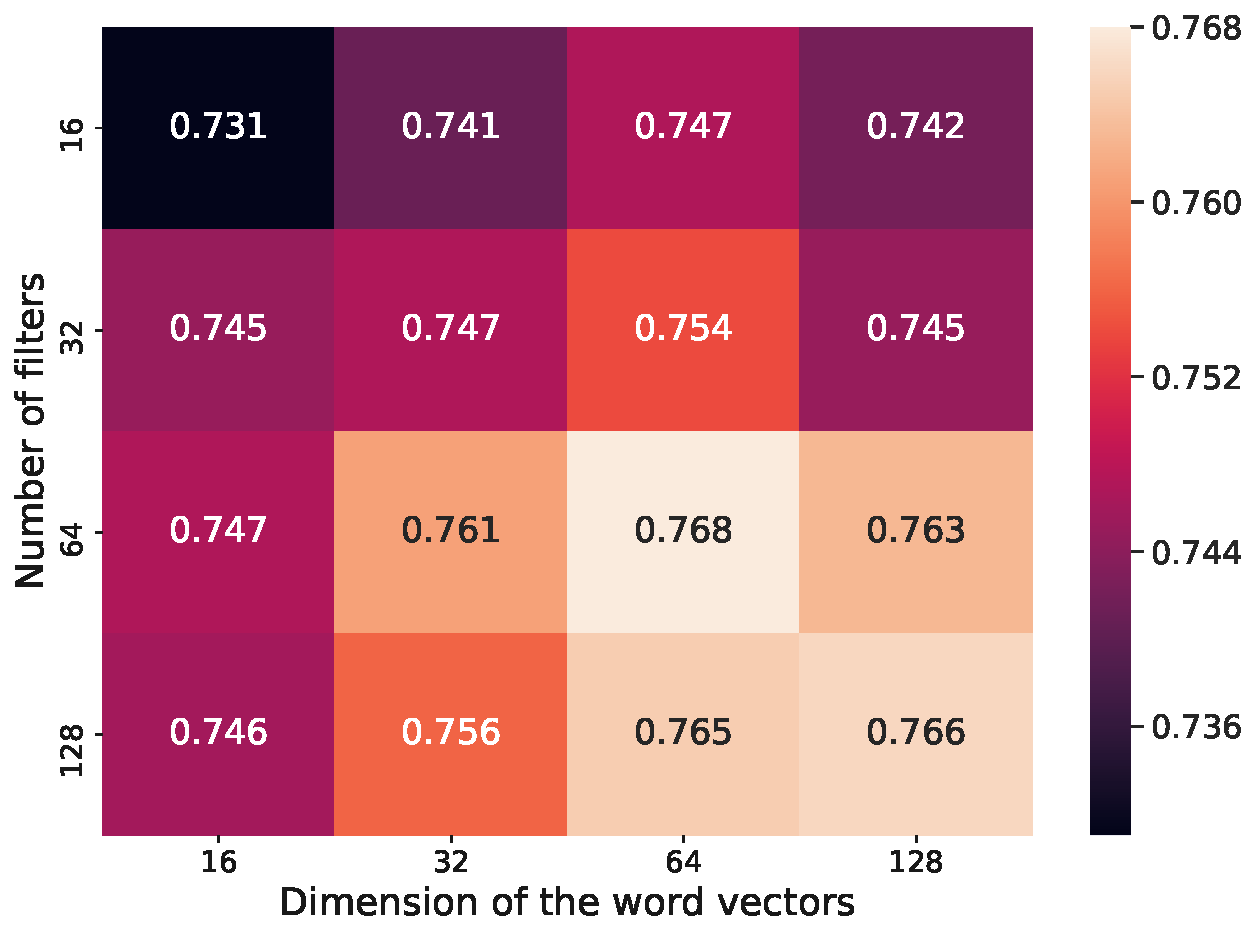
\includegraphics[width=\linewidth]{figs/QT.pdf}
    \caption{The AUC results of DeepJIT across two different hyperparameters in QT project.}
    \label{fig:qt}
\end{figure}
\begin{figure}[t!]
    \center
    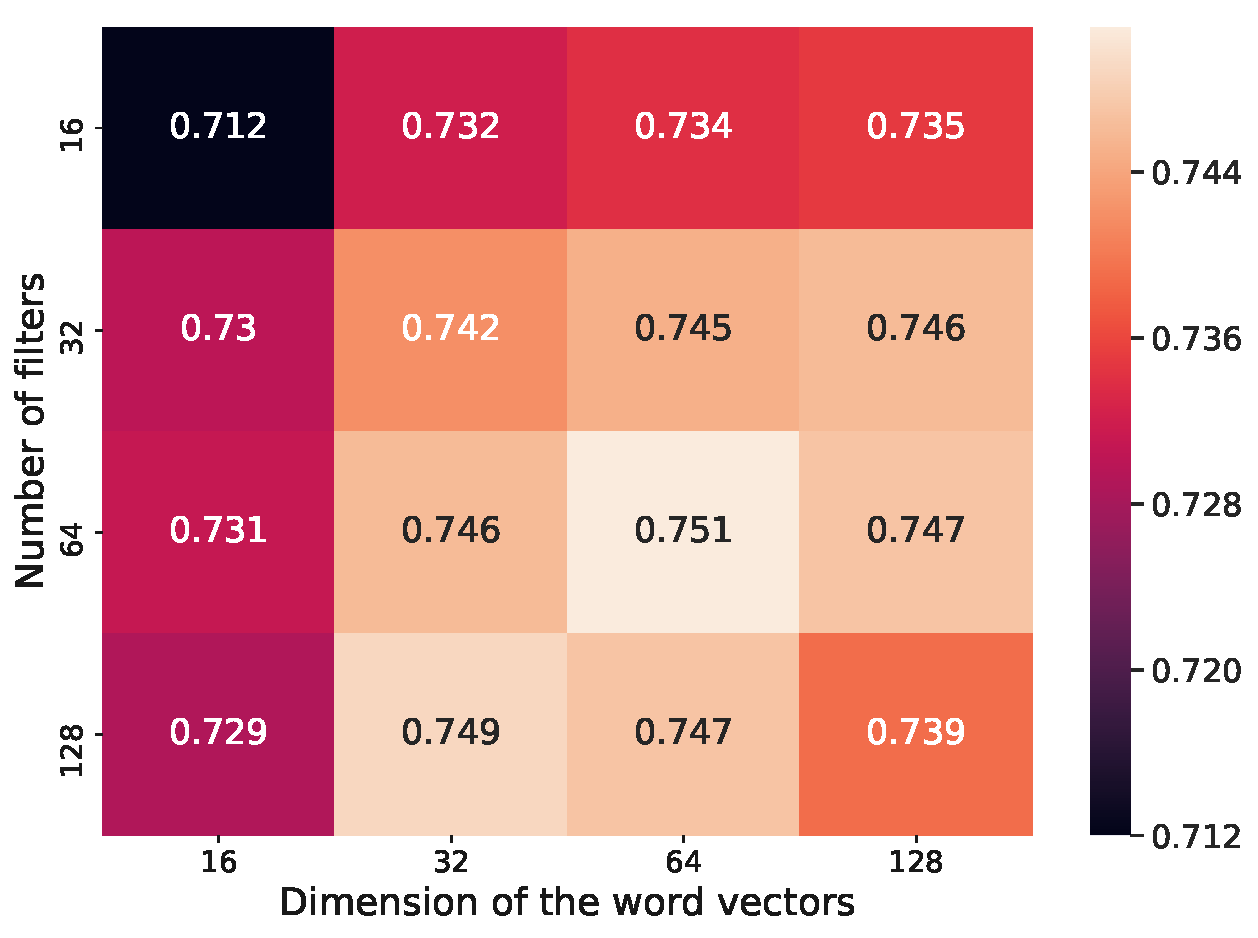
\includegraphics[width=\linewidth]{figs/OPENSTACK.pdf}
    \caption{The AUC results of DeepJIT across two different hyperparameters in OPENSTACK project.}
    \label{fig:openstack}
\end{figure}

One of the key challenge in training DeepJIT is how to select the dimension of the word vectors for the commit message ($d_m$) and code changes ($d_c$) and the size of the convolution layers (i.e., see Section~\ref{sec:cnn_msg} and Section~\ref{sec:cnn_code}). We evaluate the performance of DeepJIT, using \textit{5}-fold cross validation, across different word dimensions and filters. Figure~\ref{fig:qt} and Figure~\ref{fig:openstack} present the AUC results of DeepJIT of these hyperparameters. The figures show that the AUC achieves best results when the number of dimension of word vectors and the number of filters are set to 64. We note that there are some hyperparameters which also need to be set. The batch size is set to 32. The size of DeepJIT's fully-connected layer described in Section~\ref{sec:ftr_combine} is set to 512. We train DeepJIT using Adam~\cite{kingma2014adam} with shuffled mini-batches. We also train DeepJIT for 100 epochs. We apply the early stopping strategy~\cite{prechelt1998automatic, caruana2001overfitting} to avoid overfitting problem during the training process. Typically, we stop the training if the value of the objective function (see Equation~\ref{eq:cost}) has not been update in the last 5 epochs. All the hyperparameters in our paper are widely used in the deep learning community~\cite{severyn2015learning, huo2016learning, huo2017enhancing, hinton2012improving}.

% For the size of the convolutional filters, we choose 64. The size of DeepJIT's fully-connected layer described in Section~\ref{sec:ftr_combine} is set to 512. The word vectors dimension of the commit message ($d_m$) and code changes ($d_c$) are set to 64. We train DeepJIT using Adam~\cite{kingma2014adam} with shuffled mini-batches.  The batch size is set to 32. We train DeepJIT for 100 epochs. We also apply the early stopping strategy~\cite{prechelt1998automatic, caruana2001overfitting} to avoid overfitting problem during the training process. Typically, we stop the training if the value of the objective function (see Equation~\ref{eq:cost}) has not been update in the last 5 epochs. All these hyperparameters in our paper are widely used in the deep learning community~\cite{severyn2015learning, huo2016learning, huo2017enhancing, hinton2012improving}. 
 
 

\subsection{Research Questions and Results}
\label{sec:rq_results}

\noindent \textbf{RQ1: How effective is DeepJIT compared to the state-of-the-art baseline?}

\begin{figure}
	\center
	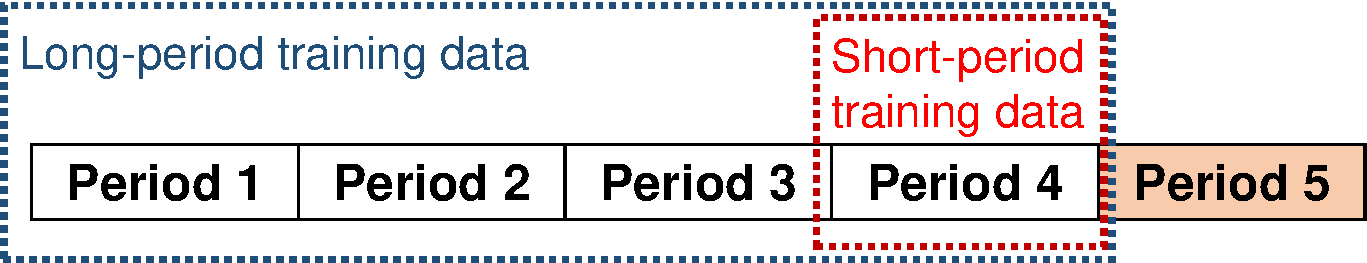
\includegraphics[scale=0.36]{figs/split.pdf}
	\caption{An example of choosing the training data for short-period and long-period models. The last period will be used as testing data.}
	\label{fig:splitting}
\end{figure}

To address RQ1, we evaluate how a JIT model, which is trained by a training data, can be used to predict buggy changes from a test data. In particular, we consider three evaluation settings: 
\begin{itemize}
\item \textbf{Cross-validation:} To evaluate machine learning algorithm, most people use $k$-fold cross-validation~\cite{kohavi1995study} in which a dataset is randomly divided to $k$ folds, each fold is considered as test data for evaluating JIT model while $k - 1$ folds are considered as train data. In this case, the JIT model is trained on a mixture of past and future data. In our paper, we set $k = 5$.
\item \textbf{Short-period:} The JIT model is trained using commits that occurred at one time period. We assume that older commits changes may have characteristics that no longer effects to the latest commits. 
\item \textbf{Long-period:} Inspired by the work~\cite{rahman2013sample}, suggesting that larger amounts of training data tend to achieve a better performance in defect prediction problem, we train the JIT model using all commits that occurred before a particular period. We discover whether additional data may improve the performance of the JIT model. 
\end{itemize} 

Figure~\ref{fig:splitting} describes how the training data is selected to train models  following the short-period and long-period settings. We use the last period (i.e., period 5) as a testing data. While the short-period model is trained using the commits that occurred during period 4, the long-period model is trained using the commits that occurred from period 1 to period 4. After training the short-period and long-period model, we measure their performance of these models using AUC described in Section~\ref{sec:metric}.

Table~\ref{tab:results} shows the AUC results of DeepJIT as well as other baselines considering the three evaluation settings: cross-validation, short-period, and long-period. The difference between results obtained using cross-validation, short-period, and long-period settings is quite small (i.e., below 2.2\%) which suggests that there is no difference between training on past or future data. 
% \cmt{TODO: Prof. Hoa, do you have any explaination about it?} 
In the QT project, DeepJIT achieves AUC scores of 0.768, 0.764, and 0.765 in three different JIT settings: cross-validation, short-period, and long-period, respectively. Comparing them to the best performing baseline (i.e., DBNJIT), DeepJIT achieves improvements of 8.96\%, 7.00\%, and 8.05\% in term of AUC. In the OPENSTACK project, DeepJIT also constitutes improvements of 8.21\%, 9.08\%, and 8.29\% in term of AUC compared to DBNJIT (the best performing baseline). We also employ the Scott-Knott test~\cite{ghotra2015revisiting} on the cross-validation setting to statistically compared the differences between the three considered JIT models. The results show that DeepJIT consistently appears in the top Scott-Knott ESD rank in term of AUC (i.e, DeepJIT $>$ DBNJIT $>$ JIT).  

\begin{table*}[t!]
	\centering
	\caption{The AUC results of DeepJIT vs. with other baselines in three types of JIT models: random, short-period, and long-period.}
	\begin{tabular}{|l|c|c|c|c|c|c|}
		\hline
		\multirow{2}[4]{*}{} & \multicolumn{3}{c|}{QT} & \multicolumn{3}{c|}{OPENSTACK} \\
		\cline{2-7}          & \textbf{Cross-validation} & \textbf{Short-period} & \textbf{Long-period} & \textbf{Cross-validation} & \textbf{Short-period} & \textbf{Long-period} \\
		\hline
		\hline
		JIT   & 0.701 & 0.703 & 0.702 & 0.691 & 0.711 & 0.706 \\
		\hline
		DBNJIT & 0.705 & 0.714 & 0.708 & 0.694 & 0.716 & 0.712 \\
		\hline
		DeepJIT & \textbf{0.768} & \textbf{0.764} & \textbf{0.765} & \textbf{0.751} & \textbf{0.781} & \textbf{0.771} \\
		\hline
	\end{tabular}%
	\label{tab:results}%
\end{table*}%

\noindent \textbf{RQ2: Does the proposed model benefit from both commit message and the code changes?}

To answer this question, we employ an ablation test~\cite{korbar2017deep, liu2017deep}, by ignoring the commit message and the code change in a commit and then evaluate the AUC performance. Specifically, we create two different variants of DeepJIT, namely DeepJIT-Msg and DeeJIT-Code. DeepJIT-Msg only considers commit message information while DeepJIT-Code only uses commit code information. We again use the three types of model settings (i.e., random, short-period, and long period) and the AUC scores to evaluate the performance of our models. Table~\ref{tab:variants} shows the performance of DeepJIT degrades if we ignore any one of the considered types of information (i.e., commit message or code changes). The AUC scores drop by 19.81\%, 28.45\%, and 19.01\% in the project QT and drop by 9.00\%, 33.96\%, and 16.00\% in the project OPENSTACK on the three types of JIT models if we ignore commit messages. The AUC scores drop by 4.07\%, 4.09\%, and 5.23\% in the project QT and drop by 3.02\%, 1.56\%, and 4.47\% in the project OPENSTACK on the three types of JIT models if we ignore code changes information. It suggests that each kind of information contributes to DeepJIT's performance. Moreover, it also indicates that the code changes are more important to detect defects in a commit than the commit message information. 

\begin{table*}[t!]
  \centering
  \caption{Contribution of feature components in DeepJIT.}
    \begin{tabular}{|l|c|c|c|c|c|c|}
    \hline
    \multirow{2}[4]{*}{} & \multicolumn{3}{c|}{QT} & \multicolumn{3}{c|}{OPENSTACK} \\
\cline{2-7}          & \multicolumn{1}{l|}{\textbf{Cross-validation}} & \multicolumn{1}{l|}{\textbf{Short-period}} & \multicolumn{1}{l|}{\textbf{Long-period}} & \multicolumn{1}{l|}{\textbf{Cross-validation}} & \multicolumn{1}{l|}{\textbf{Short-period}} & \multicolumn{1}{l|}{\textbf{Long-period}} \\
    \hline
    \hline
    DeepJIT-Msg & 0.641 & 0.609 & 0.638 & 0.689 & 0.583 & 0.659 \\
    \hline
    DeepJIT-Code & 0.738 & 0.734 & 0.727 & 0.729 & 0.769 & 0.738 \\
    \hline
    DeepJIT & \textbf{0.768} & \textbf{0.764} & \textbf{0.765} & \textbf{0.751} & \textbf{0.781} & \textbf{0.771} \\
    \hline
    \end{tabular}%
  \label{tab:variants}%

\end{table*}%

\noindent \textbf{RQ3: Does DeepJIT benefit from the manually extracted code changes features?}

\begin{table*}[t!]
  \centering
  \caption{Combination of DeepJIT with the manually code features from~\cite{mcintosh2018fix}.}
    \begin{tabular}{|l|c|c|c|c|c|c|}
    \hline
    \multirow{2}[4]{*}{} & \multicolumn{3}{c|}{QT} & \multicolumn{3}{c|}{OPENSTACK} \\
\cline{2-7}          & \textbf{Cross-validation} & \textbf{Short-period} & \textbf{Long-period} & \textbf{Cross-validation} & \textbf{Short-Period} & \textbf{Long-period} \\
    \hline
    \hline
    DeepJIT & 0.768 & 0.764 & 0.765 & 0.751 & 0.781 & 0.771  \\
    \hline
    DeepJIT-Combined & \textbf{0.779} & \textbf{0.788} & \textbf{0.786}  & \textbf{0.760} & \textbf{0.814} & \textbf{0.799} \\
    \hline
    \end{tabular}%
  \label{tab:combined}%
\end{table*}%

To address this question, we incorporate the code features, derived from~\cite{mcintosh2018fix}, into our proposed model. Specifically, the code features, namely $\textbf{z}_\textbf{r}$, are concatenated with the two embedding vectors  $\textbf{z}_\textbf{m}$ and $\textbf{z}_C$, representing the salient features of commit message and code change (see Section~\ref{sec:ftr_combine}), to build a new single vector $\textbf{z}$ as follows:
\begin{equation}
\label{eq:combined_ftr}
\textbf{z} = \textbf{z}_\textbf{m} \oplus \textbf{z}_C \oplus \textbf{z}_\textbf{r}
\end{equation}
where $\oplus$ is the concatenation operator. Table~\ref{tab:combined} shows the AUC results of DeepJIT combining with the code features. The AUC scores increase by 1.43\%, 3.14\%, and 2.75\% in the project QT and increase by 1.20\%, 4.23\%, and 3.63\% in the project OPENSTACK on the three types of JIT models settings (i.e., random, short-period, long-period). Compared to the best baseline model (i.e., DBNJIT), DeepJIT constitutes improvements of 10.50\%, 10.36\%, and 11.02\% in the project QT and 9.51\%, 13.69\%, 12.22\% in the project OPENSTACK. It suggests that the manually extracted code features are important and can be used to improve the performance of JIT's models.

\noindent \textbf{RQ4: How are the time costs of DeepJIT?}
% \begin{table*}[t!]
%   \centering
%   \caption{Time costs of DeepJIT.}
%     \begin{tabular}{|c|c|c|c|c|c|c|}
%     \hline
%     \multicolumn{1}{|c|}{\multirow{2}[4]{*}{Dataset}} & \multicolumn{2}{c|}{\textbf{Cross-validation}} & \multicolumn{2}{c|}{\textbf{Short-period}} & \multicolumn{2}{c|}{\textbf{Long-period}} \\
% \cline{2-7}          & Training time & Testing time & Training time & Testing time & Training time & Testing time \\
%     \hline
%     \hline
%     QT    & 5 hours 43 mins & 36.2 mins & 17.2 mins & 3.2 mins & 1 hours 18 mins & 8.1 mins \\
%     \hline
%     OPENSTACK & 12 hours 15 mins & 1 hours 6 mins & 10.1 mins & 2.3 mins & 2 hours 37 mins & 12.4 mins \\
%     \hline
%     \end{tabular}%
%   \label{tab:cost}%
% \end{table*}%

\begin{table}[t!]
  \centering
  \caption{Training time of DeepJIT}
    \begin{tabular}{|l|c|c|c|}
    \hline
    \multicolumn{1}{|c|}{Dataset} & \textbf{Cross-validation} & \textbf{Short-period} & \textbf{Long-period} \\
    \hline
    \hline
    QT    & 5 hours 43 mins & 17.2 mins & 1 hours 18 mins \\
    \hline
    OPENSTACK & 12 hours 15 mins & 10.1 mins & 2 hours 37 mins \\
    \hline
    \end{tabular}%
  \label{tab:cost}%
\end{table}%

We train and test DeepJIT on NVIDIA DGX1 with Tesla P100~\cite{gawande2018scaling}. Table~\ref{tab:cost} shows the time costs of training DeepJIT in three evaluation settings (i.e., cross-validation, short-period, and long-period) on QT and OPENSTACK. It is reasonable that the cross-validation setting requires longest training time since we do $5$-fold cross-validation to evaluate the performance of DeepJIT. Long-period setting requires more training time than short-period setting since it considers all commits occurring before a particular period. Once DeepJIT has been trained, it only takes a few milliseconds to generate the prediction score for a given commit.
% \cmt{Prof. Hoa: do you have any idea how to describe the time cost?}

